\documentclass[12pt,a4paper]{article}
\usepackage[utf8]{inputenc}
\usepackage{amsmath}
\usepackage{amssymb}
\usepackage{array}
\usepackage{geometry}
\usepackage{graphicx}
\geometry{hmargin=2cm,vmargin=2cm}
\newcommand{\deriv}{\mathrm{d}}

\title{Basic Control Experiments}
%\author{Nom du professeur}
\date{}

\begin{document}

\maketitle

\section{Objective}

In order to become familiar and autonomous with both control and experiments, several basic control strategies will be tested, first in simulation then experimentally. These control strategies include direct-drive and impedance control on three basic motions: 
\begin{itemize}
    \item static
    \item knee sinusoidal motion
    \item knee and hip sinusoidal motions
\end{itemize}

These motions trajectories will first be manually implemented, then by using the TSID framework. 

\section{Main code}

Two main codes were produced during this work : 
\begin{itemize}
    \item \texttt{main\_simu\_solo8\_tsid\_control.py}, the main code for simulation
    \item \texttt{main\_solo8\_tsid\_control.py}, the main code for experiments
\end{itemize}

The experimental code requires a mandatory string argument \texttt{-i}, which defines the interface used to connect to the robot. This interface can be found using the \texttt{ifconfig} command. 

Both codes take a mandatory argument \texttt{-exp}, which takes as an input an integer used to choose the controller used in the simulation. These controllers go from number 1 to 20, and are detailed in the next part.

Both codes take an optional boolean argument \texttt{-rc}, which adds a low-pass filter to the velocity measurement or estimation. This filter's goal is to remove or lower the cyclic noise created during the experiments. 

Finally, the experimental code takes an optional boolean argument \texttt{-mc}. When True, starts motion capture for the experiment. \newline

\textbf{Examples:} \\
\texttt{main\_simu\_solo8\_tsid\_control.py -exp 5 -rc False} \\
\texttt{main\_solo8\_tsid\_control.py -i interface0 -exp 2 -rc True -mc False}

\section{Control}

\subsection{Control strategies}

Three distinct control strategies are implemented: 
\begin{enumerate}
    \item Impedance control, without Feedforward torque;
    \item Impedance control, with Feedforward torque;
    \item Direct-Drive control.
\end{enumerate}


\subsubsection{Impedance control}

\textbf{Scheme:} \\

\begin{figure}[ht]
    \centering
    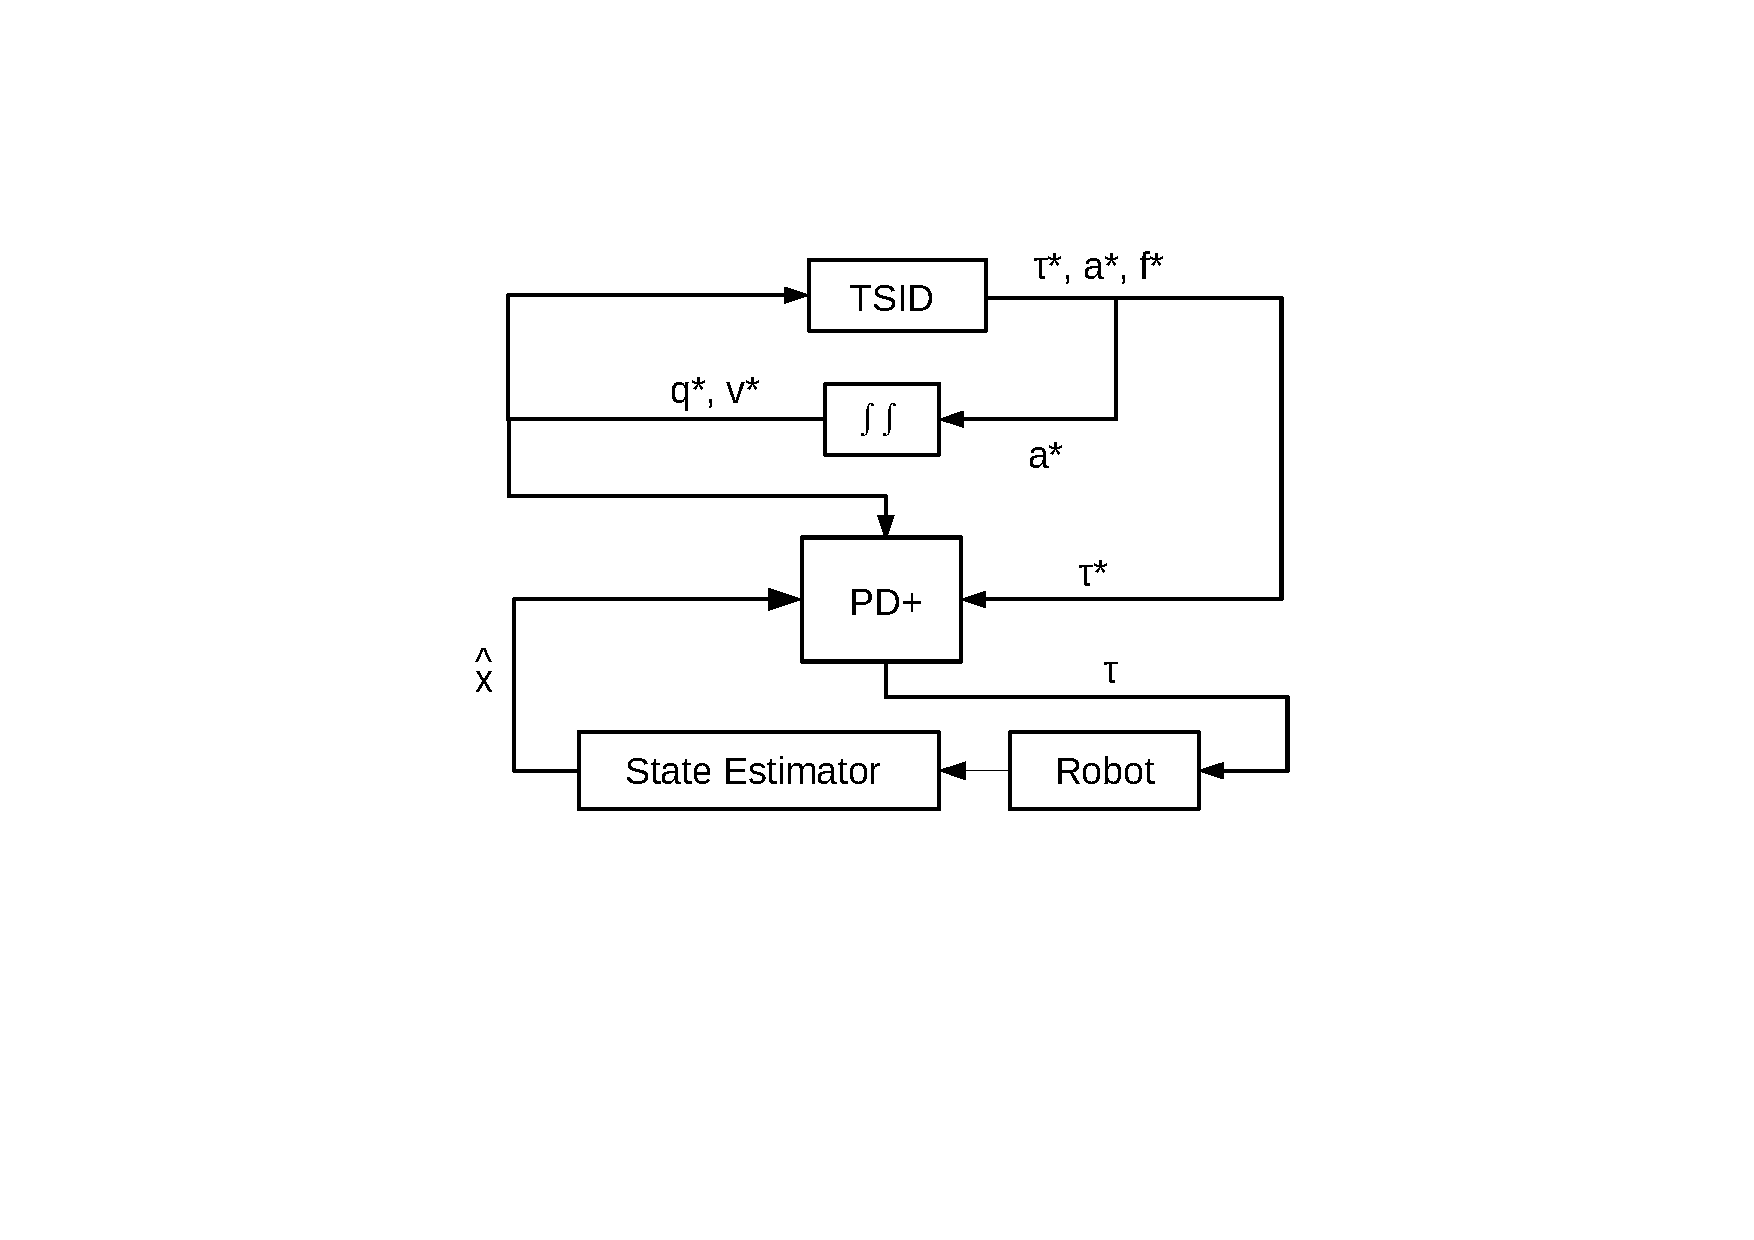
\includegraphics[width=.8\textwidth, trim = 200 180 180 120, clip]{Pics/IC_scheme.pdf}
    \caption{Impedance Control Scheme}
    \label{fig:ic_scheme}
\end{figure}

\subsubsection*{Without Feedforward}

\textbf{Torque calculation:}

\begin{equation}
    \tau = Kp (q - qmes) + Kd (v - vmes)
\end{equation}

\subsubsection*{With Feedforward}

\textbf{Torque calculation:}

\begin{equation}
    \tau = Kp (q - qmes) + Kd (v - vmes) + \tau_{FF}
\end{equation}

with
\begin{equation}
    \tau_{FF} = 
    \left\{
    \begin{tabular}{l l}
         \texttt{pinocchio.rnea(model, data, q, v, dv)} & \text{if the motion is manually generated}\\
         \texttt{tsid.getActuatorForces(sol)} & \text{if the motion is generated by TSID} 
    \end{tabular}
    \right.
\end{equation}

\subsubsection{Direct-drive control}

\textbf{Schematic:}

\begin{figure}[ht]
    \centering
    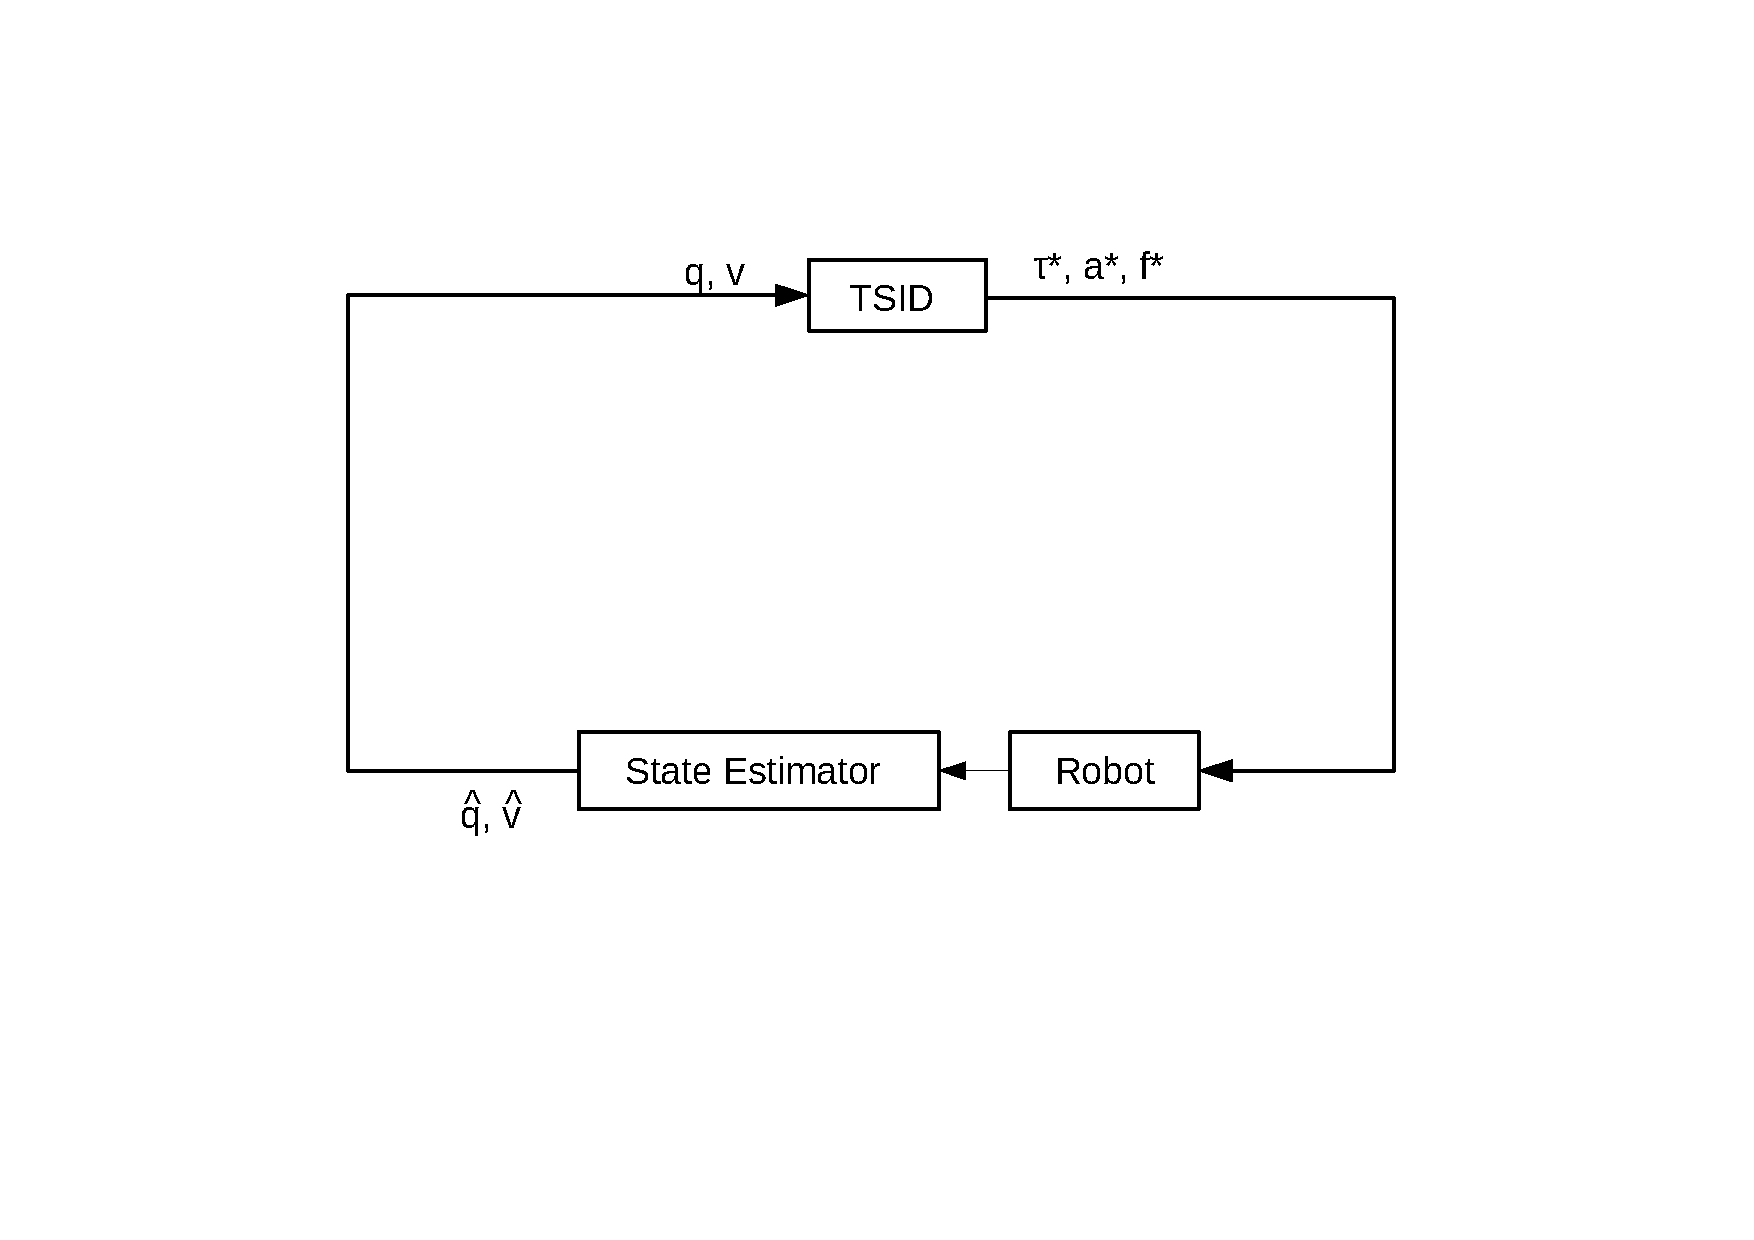
\includegraphics[width=.8\textwidth, trim = 150 180 150 120, clip]{Pics/DTC_scheme.pdf}
    \caption{Direct-Drive Control Scheme}
    \label{fig:ddc_scheme}
\end{figure}

\subsection{Motions}

In order to test these control strategies, four motions are studied: 
\begin{enumerate}
    \item the robot remaining static,
    \item a sinusoidal motion of the front left knee,
    \item a small sinusoidal motion of the front left hip and knee,
    \item a wide sinusoidal motion of the front left hip and knee.
\end{enumerate}
These motions can either be generated manually, or generated by inverse dynamics calculations with TSID, by creating posture tasks.

\subsection{Controllers}

These controllers from 1 to 20 are detailed in the following sections.

\subsubsection{Controller 1}

\textbf{Control Strategy:} Impedance control without feedforward \\
\textbf{Type of motion:} Static \\
\textbf{Motion generation:} Manual \\
\textbf{Simulation:} \texttt{python3 main\_simu\_solo8\_tsid\_control.py -exp 1} \\
\textbf{Experiment:} \texttt{sudo -E python3 main\_solo8\_tsid\_control.py -i interface\_name -exp 1} \\

\subsubsection{Controller 2}

\textbf{Control Strategy:} Impedance control without feedforward \\
\textbf{Type of motion:} Sinusoidal knee motion \\
\textbf{Motion generation:} Manual \\
\textbf{Simulation:} \texttt{python3 main\_simu\_solo8\_tsid\_control.py -exp 2} \\
\textbf{Experiment:} \texttt{sudo -E python3 main\_solo8\_tsid\_control.py -i interface\_name -exp 2} \\

\subsubsection{Controller 3}

\textbf{Control Strategy:} Impedance control without feedforward \\
\textbf{Type of motion:} Small sinusoidal hip and knee motions \\
\textbf{Motion generation:} Manual \\
\textbf{Simulation:} \texttt{python3 main\_simu\_solo8\_tsid\_control.py -exp 3} \\
\textbf{Experiment:} \texttt{sudo -E python3 main\_solo8\_tsid\_control.py -i interface\_name -exp 3} \\

\subsubsection{Controller 4}

\textbf{Control Strategy:} Impedance control without feedforward \\
\textbf{Type of motion:} Wide sinusoidal hip and knee motions \\
\textbf{Motion generation:} Manual \\
\textbf{Simulation:} \texttt{python3 main\_simu\_solo8\_tsid\_control.py -exp 4} \\
\textbf{Experiment:} \texttt{sudo -E python3 main\_solo8\_tsid\_control.py -i interface\_name -exp 4} \\

\subsubsection{Controller 5}

\textbf{Control Strategy:} Impedance control with feedforward \\
\textbf{Type of motion:} Static \\
\textbf{Motion generation:} Manual \\
\textbf{Simulation:} \texttt{python3 main\_simu\_solo8\_tsid\_control.py -exp 5} \\
\textbf{Experiment:} \texttt{sudo -E python3 main\_solo8\_tsid\_control.py -i interface\_name -exp 5} \\

\subsubsection{Controller 6}

\textbf{Control Strategy:} Impedance control with feedforward \\
\textbf{Type of motion:} Sinusoidal knee motion \\
\textbf{Motion generation:} Manual \\
\textbf{Simulation:} \texttt{python3 main\_simu\_solo8\_tsid\_control.py -exp 6} \\
\textbf{Experiment:} \texttt{sudo -E python3 main\_solo8\_tsid\_control.py -i interface\_name -exp 6} \\

\subsubsection{Controller 7}

\textbf{Control Strategy:} Impedance control with feedforward \\
\textbf{Type of motion:} Small sinusoidal hip and knee motions \\
\textbf{Motion generation:} Manual \\
\textbf{Simulation:} \texttt{python3 main\_simu\_solo8\_tsid\_control.py -exp 7} \\
\textbf{Experiment:} \texttt{sudo -E python3 main\_solo8\_tsid\_control.py -i interface\_name -exp 7} \\

\subsubsection{Controller 8}

\textbf{Control Strategy:} Impedance control with feedforward \\
\textbf{Type of motion:} Wide sinusoidal hip and knee motions \\
\textbf{Motion generation:} Manual \\
\textbf{Simulation:} \texttt{python3 main\_simu\_solo8\_tsid\_control.py -exp 8} \\
\textbf{Experiment:} \texttt{sudo -E python3 main\_solo8\_tsid\_control.py -i interface\_name -exp 8} \\

\subsubsection{Controller 9}

\textbf{Control Strategy:} Impedance control without feedforward \\
\textbf{Type of motion:} Static \\
\textbf{Motion generation:} TSID \\
\textbf{Simulation:} \texttt{python3 main\_simu\_solo8\_tsid\_control.py -exp 9} \\
\textbf{Experiment:} \texttt{sudo -E python3 main\_solo8\_tsid\_control.py -i interface\_name -exp 9} \\

\subsubsection{Controller 10}

\textbf{Control Strategy:} Impedance control without feedforward \\
\textbf{Type of motion:} Sinusoidal knee motion \\
\textbf{Motion generation:} TSID \\
\textbf{Simulation:} \texttt{python3 main\_simu\_solo8\_tsid\_control.py -exp 10} \\
\textbf{Experiment:} \texttt{sudo -E python3 main\_solo8\_tsid\_control.py -i interface\_name -exp 10} \\

\subsubsection{Controller 11}

\textbf{Control Strategy:} Impedance control without feedforward \\
\textbf{Type of motion:} Small sinusoidal hip and knee motions \\
\textbf{Motion generation:} TSID \\
\textbf{Simulation:} \texttt{python3 main\_simu\_solo8\_tsid\_control.py -exp 11} \\
\textbf{Experiment:} \texttt{sudo -E python3 main\_solo8\_tsid\_control.py -i interface\_name -exp 11} \\

\subsubsection{Controller 12}

\textbf{Control Strategy:} Impedance control without feedforward \\
\textbf{Type of motion:} Wide sinusoidal hip and knee motions \\
\textbf{Motion generation:} TSID \\
\textbf{Simulation:} \texttt{python3 main\_simu\_solo8\_tsid\_control.py -exp 12} \\
\textbf{Experiment:} \texttt{sudo -E python3 main\_solo8\_tsid\_control.py -i interface\_name -exp 12} \\

\subsubsection{Controller 13}

\textbf{Control Strategy:} Impedance control with feedforward \\
\textbf{Type of motion:} Static \\
\textbf{Motion generation:} TSID \\
\textbf{Simulation:} \texttt{python3 main\_simu\_solo8\_tsid\_control.py -exp 13} \\
\textbf{Experiment:} \texttt{sudo -E python3 main\_solo8\_tsid\_control.py -i interface\_name -exp 13} \\

\subsubsection{Controller 14}

\textbf{Control Strategy:} Impedance control with feedforward \\
\textbf{Type of motion:} Sinusoidal knee motion \\
\textbf{Motion generation:} TSID \\
\textbf{Simulation:} \texttt{python3 main\_simu\_solo8\_tsid\_control.py -exp 14} \\
\textbf{Experiment:} \texttt{sudo -E python3 main\_solo8\_tsid\_control.py -i interface\_name -exp 14} \\

\subsubsection{Controller 15}

\textbf{Control Strategy:} Impedance control with feedforward \\
\textbf{Type of motion:} Small sinusoidal hip and knee motions \\
\textbf{Motion generation:} TSID \\
\textbf{Simulation:} \texttt{python3 main\_simu\_solo8\_tsid\_control.py -exp 15} \\
\textbf{Experiment:} \texttt{sudo -E python3 main\_solo8\_tsid\_control.py -i interface\_name -exp 15} \\

\subsubsection{Controller 16}

\textbf{Control Strategy:} Impedance control with feedforward \\
\textbf{Type of motion:} Wide sinusoidal hip and knee motions \\
\textbf{Motion generation:} TSID \\
\textbf{Simulation:} \texttt{python3 main\_simu\_solo8\_tsid\_control.py -exp 16} \\
\textbf{Experiment:} \texttt{sudo -E python3 main\_solo8\_tsid\_control.py -i interface\_name -exp 16} \\

\subsubsection{Controller 17}

\textbf{Control Strategy:} Direct-drive control \\
\textbf{Type of motion:} Static \\
\textbf{Motion generation:} TSID \\
\textbf{Simulation:} \texttt{python3 main\_simu\_solo8\_tsid\_control.py -exp 17} \\
\textbf{Experiment:} \texttt{sudo -E python3 main\_solo8\_tsid\_control.py -i interface\_name -exp 17} \\

\subsubsection{Controller 18}

\textbf{Control Strategy:} Direct-drive control \\
\textbf{Type of motion:} Sinusoidal knee motion \\
\textbf{Motion generation:} TSID \\
\textbf{Simulation:} \texttt{python3 main\_simu\_solo8\_tsid\_control.py -exp 18} \\
\textbf{Experiment:} \texttt{sudo -E python3 main\_solo8\_tsid\_control.py -i interface\_name -exp 18} \\

\subsubsection{Controller 19}

\textbf{Control Strategy:} Direct-drive control \\
\textbf{Type of motion:} Small sinusoidal hip and knee motions \\
\textbf{Motion generation:} TSID \\
\textbf{Simulation:} \texttt{python3 main\_simu\_solo8\_tsid\_control.py -exp 19} \\
\textbf{Experiment:} \texttt{sudo -E python3 main\_solo8\_tsid\_control.py -i interface\_name -exp 19} \\

\subsubsection{Controller 20}

\textbf{Control Strategy:} Direct-drive control \\
\textbf{Type of motion:} Wide sinusoidal hip and knee motions \\
\textbf{Motion generation:} TSID \\
\textbf{Simulation:} \texttt{python3 main\_simu\_solo8\_tsid\_control.py -exp 20} \\
\textbf{Experiment:} \texttt{sudo -E python3 main\_solo8\_tsid\_control.py -i interface\_name -exp 20} \\


\subsubsection{Recap}

\begin{table}[ht]
    \centering
    \begin{tabular}{|c|c|c|c|c|c|c|}
    \hline
        \textbf{Controller} & \textbf{PD} & \textbf{PD+} & \textbf{Direct-Drive} & \textbf{Motion} & \textbf{Manual} & \textbf{TSID} \\
        \hline
        \hline
        1 & X & & & Static & X & \\
        2 & X & & & Knee & X & \\
        3 & X & & & Hip + Knee (Small) & X & \\
        4 & X & & & Hip + Knee (Wide) & X & \\
        \hline
        5 & & X & & Static & X & \\
        6 & & X & & Knee & X & \\
        7 & & X & & Hip + Knee (Small) & X & \\
        8 & & X & & Hip + Knee (Wide) & X & \\
        \hline
        9 & X & & & Static & & X \\
        10 & X & & & Knee & & X \\
        11 & X & & & Hip + Knee (Small) & & X \\
        12 & X & & & Hip + Knee (Wide) & & X \\
        \hline
        13 & & X & & Static & & X \\
        14 & & X & & Knee & & X \\
        15 & & X & & Hip + Knee (Small) & & X \\
        16 & & X & & Hip + Knee (Wide) & & X \\
        \hline
        17 & & & X & Static & & X \\
        18 & & & X & Knee & & X \\
        19 & & & X & Hip + Knee (Small) & & X \\
        20 & & & X & Hip + Knee (Wide) & & X \\
        \hline
    \end{tabular}
    \caption{Controllers recap}
    \label{tab:recap}
\end{table}



\end{document}
